\documentclass[a4paper, 12pt]{article}
\usepackage{comment} 
\usepackage{fullpage}
\usepackage[hidelinks]{hyperref}
\usepackage{amsmath}
\usepackage{graphicx}
\usepackage{environ}
\usepackage{tabto,enumitem}

\usepackage{algorithm}
\usepackage{algpseudocode}

\begin{document}
\noindent
\large\textbf{SOEN 6011 SEP} \hfill \textbf{Mahavir Patel} \\
\normalsize Problem 3 \hfill \textbf{40198619} \\
Function 6 :  $B(x,y)$ Beta Function \hfill Date: 05/07/2022 \\

\section{Algorithm 1 - Tail Recursive Factorial Function}
The gamma function is utilised by the beta function to calculate positive integers. The factorial of the number makes it simple to determine the Gamma Value of a positive integer. \\
\begin{center}
    $B(x,y)=\frac{\Gamma x \Gamma y}{\Gamma (x+y)}$ where $\Gamma x = (x-1)!$\\
\end{center}

\subsection{Advantages}
\begin{itemize}
    \item The algorithm Gives the accurate answers for the positive integers.
    \item The execution speed of the tail recursive function compared to recursive function is very fast and memory efficient. 
    \item This algorithm makes it simple to calculate the integer's beta values.
\end{itemize}
\subsection{disadvantages}
\begin{itemize}
    \item Can be used for only Positive numbers.
    \item Only calculate the Beta Values for the integer
    \item It does not Consider decimal numbers.
\end{itemize}

\subsection{Why Tail Recursive Function ?}
If a function concludes by returning the result of the recursive call, it is considered tail-recursive. It is a waste of memory to keep the caller's frame on the stack after the recursive call returns its value because nothing else has to be done. Therefore, the current frame can be used for the call rather than allocating a new one. And for the small value of the integer sometimes recursive factorial faction can cause StackOverFlow error that's why it's better to use the tail recursive function. \\

\newpage
\subsection{Algorithm}

\begin{algorithm}
\caption{Calculate Beta Function using factorial}

\textbf{Require:}  value: $x > 0$ \& $y>0$  \Comment{where $x,y \in {Z}^+$}\\
\textbf{Ensure:} $result = Beta(x,y)$
\begin{algorithmic}[1]

\Procedure {BetaFunction}{$x, y$}
    \State $value1 \leftarrow \Call{CalculateGamma}{x}$
    \State $value2 \leftarrow \Call{CalculateGamma}{y}$
    \State $value3 \leftarrow \Call{CalculateGamma}{x+y}$
    \State $betaValue \leftarrow \frac{value1 * value2}{value3}$
    \State \textbf{return} $betaValue$\Comment{It returns the beta value}
    \EndProcedure
\Statex


\Procedure {GammaFunction}{$value$}
    \State $value \leftarrow value-1$
    \State \textbf{return} $\Call{Factorial}{value}$ \Comment{It returns the gamma value}
    \EndProcedure
\Statex

\Procedure {Factorial}{$value$}
    \State \textbf{return} $\Call{FactorialTailRecursive}{value,1}$ \Comment{It returns the factorial of the number}
    \EndProcedure
\Statex

\Procedure{FactorialTailRecursive}{$value, n$}
    \If{$value = 0 $}
    \State \textbf{return} $n$ \Comment{Return factorial of the number} 
    \Else
    \State \textbf{return} \Call{FactorialTailRecursive}{$value - 1$, $value * n$ } \Comment{tail recursive call to function}
    \EndIf
    \EndProcedure
\Statex


\State $result \leftarrow \Call{CalculateBeta}{x,y} $\Comment{Final result of $Beta(x,y)$}

\end{algorithmic}
\end{algorithm}

\newpage
\section{Algorithm 2 - Stirling's approximation}
The gamma Stirling's approximation, also referred to as Stirling's formula is a mathematical approximation for factorials for decimal values and can be used to construct the beta function for decimal numbers. Since it is a good approximation, it delivers correct results even for small values of n. \\

\begin{center}
    $B(x,y)=\frac{\Gamma x \Gamma y}{\Gamma (x+y)}$ where, $\Gamma n = \sqrt{2 \pi n} \cdot (\frac{n}{e})^n$\\
\end{center}

\subsection{Advantages}
\begin{itemize}
    \item The algorithm Gives the answers for the positive real numbers.
    \item Most values that are available can be computed by the algorithm.
    \item It is possible to apply this approximation approach in place of the integration function to reduce the complexity of the code
\end{itemize}
\subsection{disadvantages}
\begin{itemize}
    \item The algorithm is unable to produce reliable answers.
    \item Although the complexity is decreased, the earlier algorithm is still substantially more difficult.
    \item The code cannot be easily debugged.
    \item The mismatch between the necessary and actual answers is much different for smaller values. However, the difference gets smaller as the size of the numbers grows.
\end{itemize}

\subsection{Why to use Stirling's Approximation ?}
To calculate the Beta value of the decimal number, it's hard to compute using the gamma integral function. However, Stirlings' approximation can be applied to reduce the complexity. Even for small numbers, this is a good approximation procedure that yields accurate answers. The best outcome is always obtained through approximation. The comparison of Stirling's approximation and the factorial is provided below.


\newpage
\subsection{Algorithm}

\begin{algorithm}
\caption{Calculate Beta Function using Stirlings's approximation}

\textbf{Require:}  value: $x > 0$ \& $y>0$  \Comment{where $x,y \in R^+$}\\
\textbf{Ensure:} $result = Beta(x,y)$
\begin{algorithmic}[1]

\Procedure {CalculateBeta}{$x, y$}
    \State $value1 \leftarrow \Call{CalculateGamma}{x}$
    \State $value2 \leftarrow \Call{CalculateGamma}{y}$
    \State $value3 \leftarrow \Call{CalculateGamma}{x+y}$
    \State $beta \leftarrow \frac{value1 * value2}{value3}$
    \State \textbf{return} $beta$\Comment{It returns the beta value}
    \EndProcedure
\Statex

\Procedure {CalculateGamma}{$value$}
    \State $firstPart \leftarrow 2 \cdot \pi \cdot value$
    \State $secondPart \leftarrow (\frac{value}{e})$
    \State $gamma \leftarrow \Call{CalculatePower}{firstPart,\frac{1}{2}} \Call{CalculatePower}{secondPart,value}$
    \State \textbf{return} $gamma$\Comment{It returns the gamma value}
    \EndProcedure
\Statex

\Procedure {CalculatePower}{$value1$,$value2$}
    \State $power \leftarrow math.power(value1,value2)$
    \State \textbf{return} $power$\Comment{It returns the base to the power}
    \EndProcedure
\Statex

\Procedure{CalculateLog}{$value$}
    \State $answer \leftarrow 0$
    \State $base \leftarrow \frac{value-1}{value+1}$
    \For {$i \leftarrow 1, 125 $}
    \State $exponent \leftarrow 2 * i - 1$
    \State $answer \leftarrow answer + \frac{1}{exponent}*\Call{calculatePower}{base,exponent}$
    \EndFor
    \State \textbf{return} $2*answer$ \Comment{It returns the value of Log n}
    \EndProcedure
\Statex
\State $result \leftarrow \Call{CalculateBeta}{x,y} $\Comment{Final result of $Beta(x,y)$}

\end{algorithmic}
\end{algorithm}

\begin{algorithm}
\caption{Calculate the power(x,y)}

\textbf{Require:}  value: $x$ \& $y$  \Comment{where $x,y \in R$}\\
\textbf{Ensure:} $result = Power(x,y)$
\begin{algorithmic}[1]

\Procedure {CalculatePower}{$base$,$exponent$}
    \State Convert the exponent into String
    \State $exponentArray \leftarrow Split\;the\;exponent\;into\;integer\;and\;fractional\;part$
    \If{$exponetArray[1] > 0$}
    \State \textbf{return} \Call{calculateFractionPower}{$base$,$exponent$}
    \EndIf
    %\State $value2 \leftarrow value-1$
    \If{$exponent < 0 $}
    \State $base \leftarrow \frac{1}{base}$
    \State $exponent \leftarrow (-1) \cdot exponent$
    \EndIf
    \If{$exponent \leftarrow 0$}
    \State \textbf{return} 1
    \EndIf
    \If{$exponent \% 2 \leftarrow 0$}
    \State $base \leftarrow base * base$
    \State $exponent \leftarrow \frac{exponent}{2}$
    \State \textbf{return} \Call{calculatePower}{$base$,$exponent$}
    \Else
    \State $exponent \leftarrow \frac{exponent-1}{2}$
    \State \textbf{return} $base$ * $\Call{calculatePower}{base*base,exponent}$
    \EndIf
    \EndProcedure
\Statex


\Procedure {CalculateFractionPower}{$base$,$exponent$}
    \State $answer \leftarrow 0$
    \State $logvalue \leftarrow 0$
    \If{$exponet \leftarrow 0$}
    \State \textbf{return} 1
    \EndIf
    \If{$base < 0 $}
    \State $logvalue \leftarrow \Call{calculateLog}{base * (-1)}$
    \Else
    \State $logvalue \leftarrow \Call{calculateLog}{base}$
    \EndIf
    \If{$exponent \leftarrow 0 \land exponent > 0$}
    \State \textbf{return} $answer$
    \EndIf
    \For {$i \leftarrow 0, 125 $}
    \State $numerator \leftarrow \Call{calculatePower}{exponent*logvalue,i}$
    \State $denominator \leftarrow \Call{Factorial}{i}$
    \State $answer \leftarrow answer + \frac{numerator}{denominator}$
    \EndFor
    
    \If{$base < 0 \land \;exponent \% 2 \neq 0$}
    \State \textbf{return} $answer * (-1)$
    \Else
    \State \textbf{return} $answer$
    \EndIf
    \EndProcedure
\Statex

\end{algorithmic}
\end{algorithm}

\newpage

\section{Mind Map}

\begin{figure}[h]
    \centering
    \begin{center}
    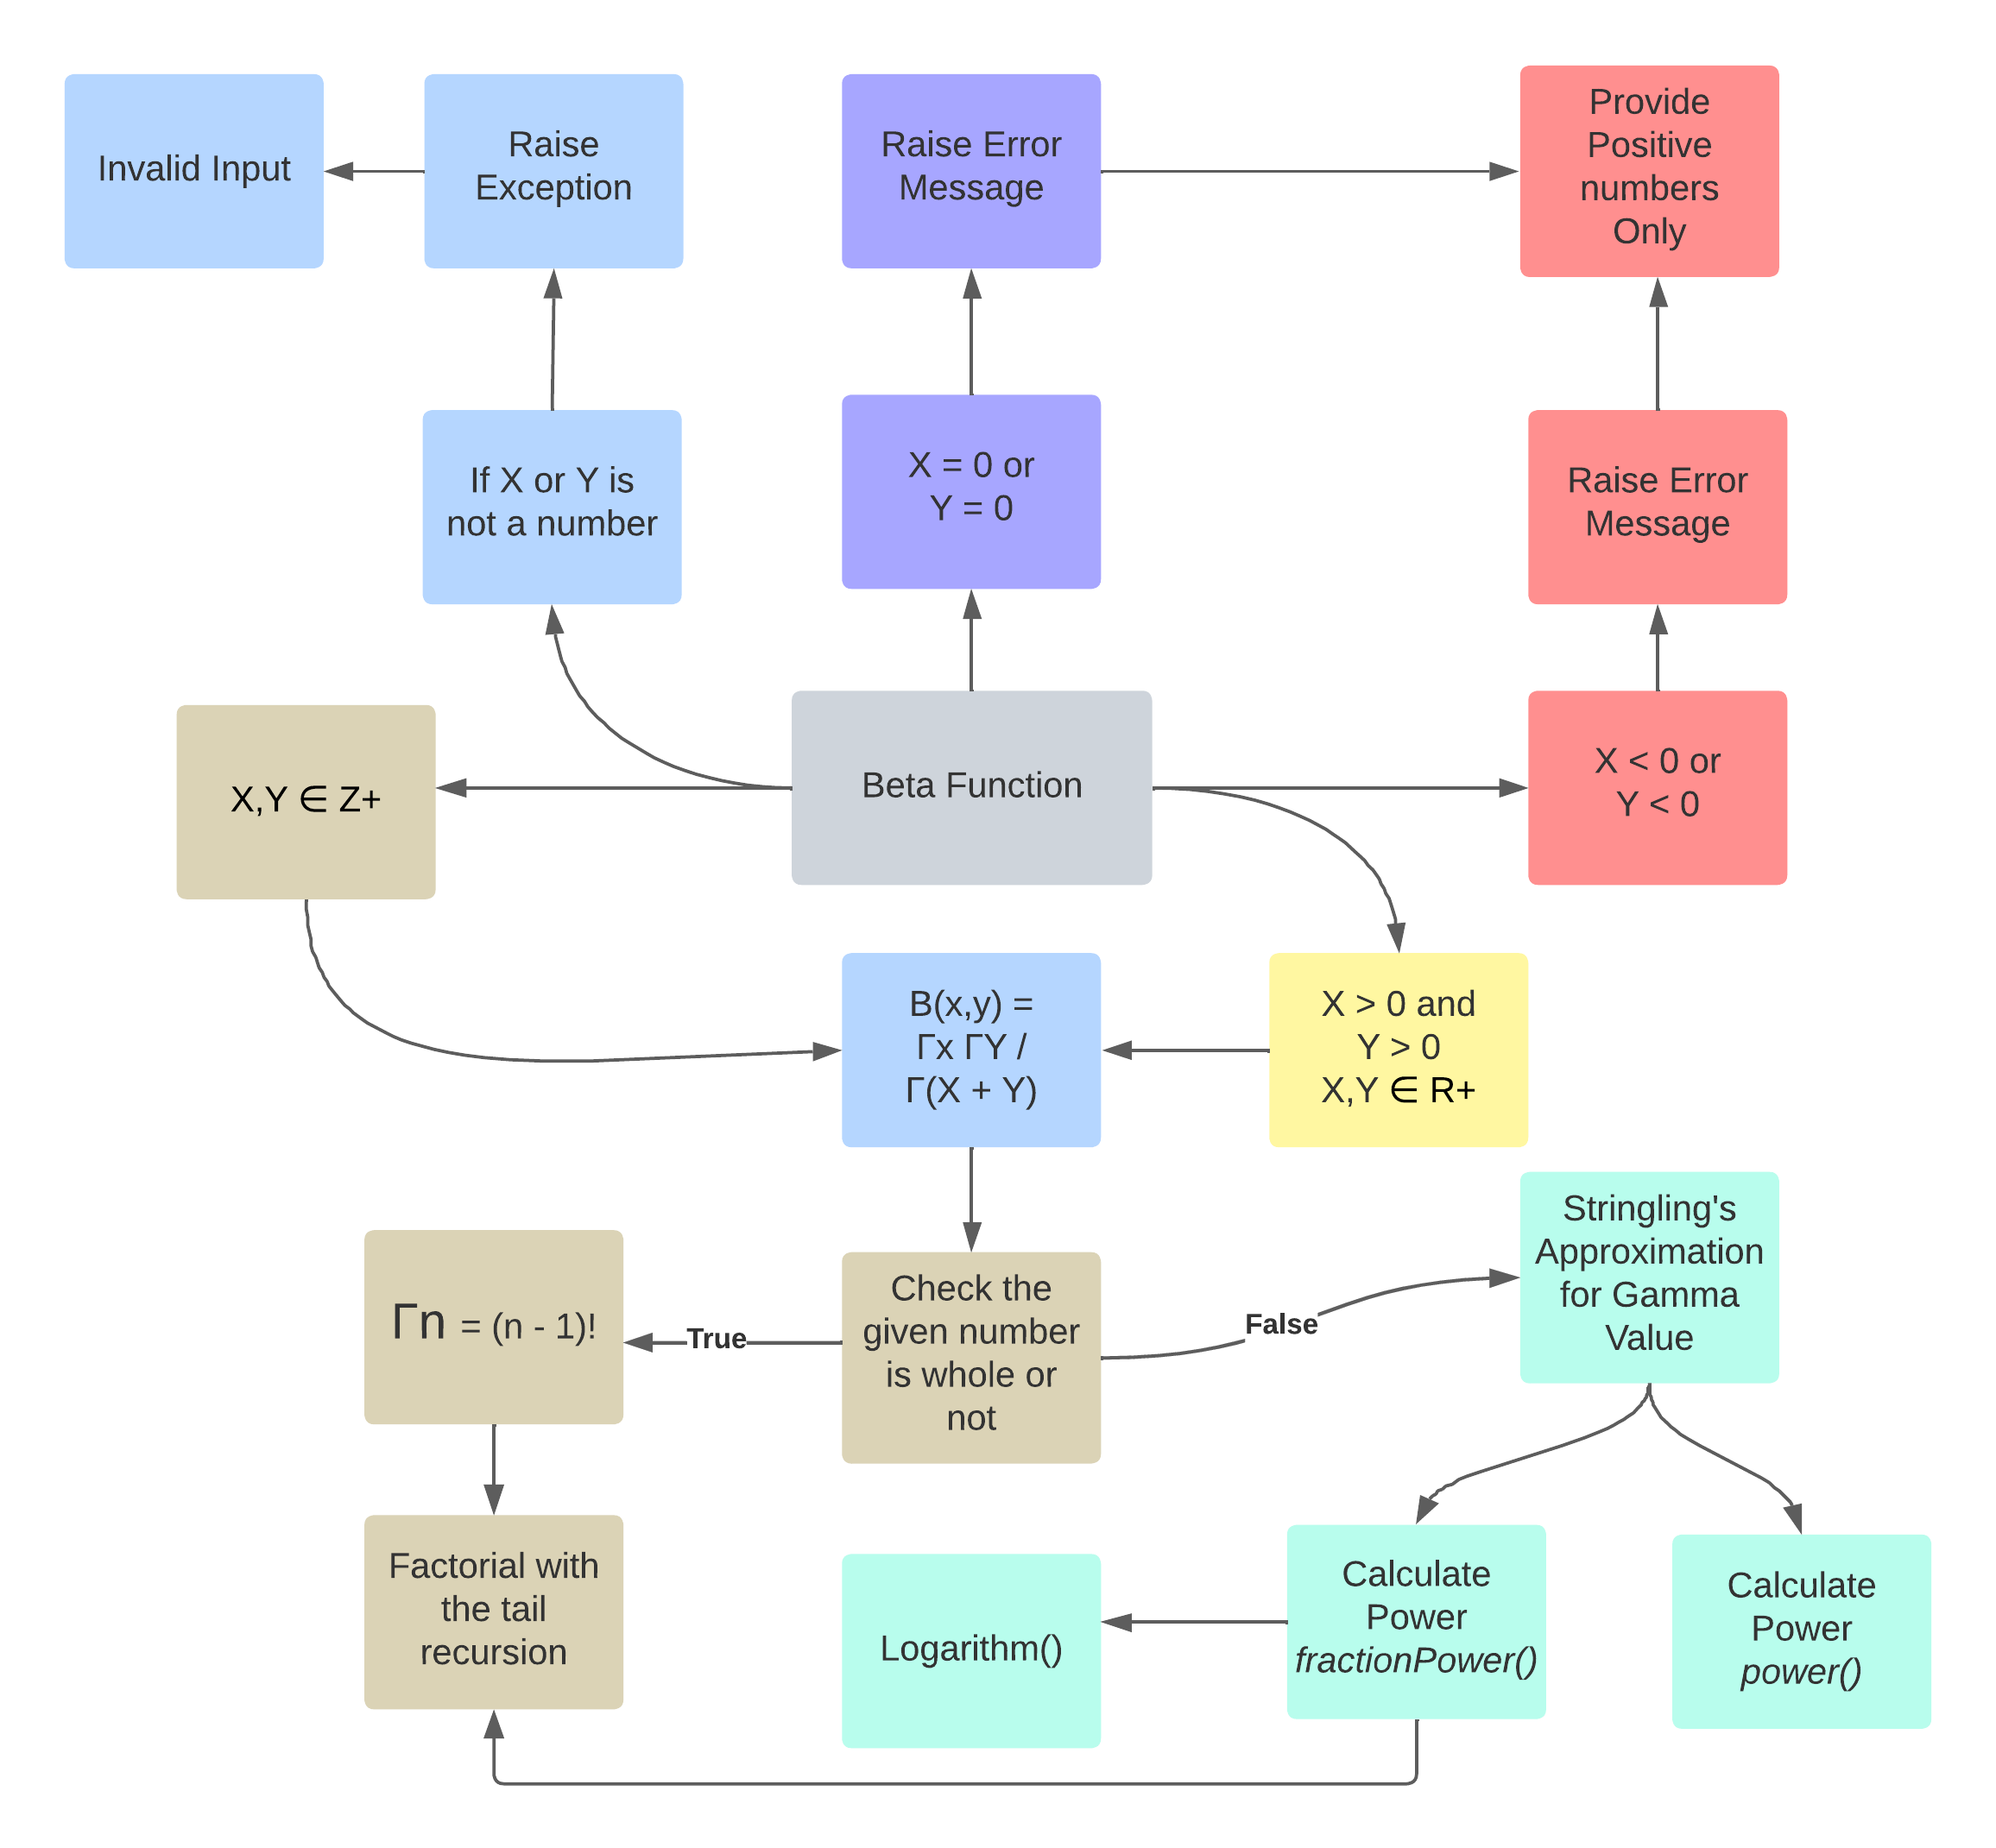
\includegraphics[width=1.0\linewidth]{Images/Mind-Map.png}    
    \end{center}
    \caption{Mind Map for Pseudo Code}
    \label{fig:Mind Map}
\end{figure}


\newpage

\begin{thebibliography}{15}

\addcontentsline{toc}{chapter}{Bibliography}
\bibitem{1}
Beta Function WikiPedia
\\\href{https://en.wikipedia.org/wiki/Beta\_function}{https://en.wikipedia.org/wiki/Beta\_function}

\bibitem{2}
Stirling's Approximation
\\\href{https://en.wikipedia.org/wiki/Stirling\%27s\_approximation}{https://en.wikipedia.org/wiki/Stirling\%27s\_approximation}

\bibitem{3}
Tail Recursion
\\\href{https://www.geeksforgeeks.org/tail-recursion/}{https://www.geeksforgeeks.org/tail-recursion/}

\end{thebibliography}


\end{document}
